\documentclass{beamer}

\newtheorem{defn}{Definition}

\begin{document}

\begin{frame}
    \title{Review of chapter2 $\sim$  chapter6}
    \titlepage.
\end{frame}

\begin{frame}{Chapter2 $\sim$ Chapter3}
    \begin{enumerate}
        \item Data features:
            \begin{itemize}
                \item Domain set: set of objects $ \mathcal{X} $
                \item Label set: set of objects $ \mathcal{Y} $
                \item Unknown distribution: 
                    \begin{itemize}
                        \item $ \mathcal{D} \sim \mathcal{X}$, with unknown fixed mapping function $f: \mathcal{X} \rightarrow \mathcal{Y} $
                        \item $ \mathcal{D} \sim (\mathcal{X}, \mathcal{Y}) $
                    \end{itemize}
                \item Training data: finite sequence $ S = \mathcal{X} \times \mathcal{Y} = \{(x_1, y_1), (x_2, y_2), \dots, (x_m, y_m) \}$
            \end{itemize}
        \item Learning framework:
            \begin{itemize}
                \item Label function: $ h: \mathcal{X} \rightarrow \mathcal{Y} $
                \item Hypothesis set (or Hypothesis class): $ \mathcal{H} = \{ h_1, h_2, \dots \} $
                \item True error:
                    $ L_{\mathcal{D}}(h) := \underset{(x,y) \thicksim \mathcal{D}}{\mathbb{P}}[h(x)\ne y]:=\mathcal{D}(\{(x,y) : h(x)\ne y\})​$
                \item Empirical error:
                    $L_s(h) := \frac{|\{ i \in [m] : h(x_i)\ne y_i\}|}{m}, [m]=\{1,\ldots ,m\}​$
                \item Empirical risk minimization:
                    $ h^{ERM}_S = \arg\min_{h \in \mathcal{H}} L_S(h) $
                \item ERM algorithm: $A^{ERM}: S \rightarrow h^{ERM}_S $
            \end{itemize}
    \end{enumerate}
\end{frame}

\begin{frame}{Chapter2 $\sim$ Chapter3}
    \begin{figure}[h]
        \centering
        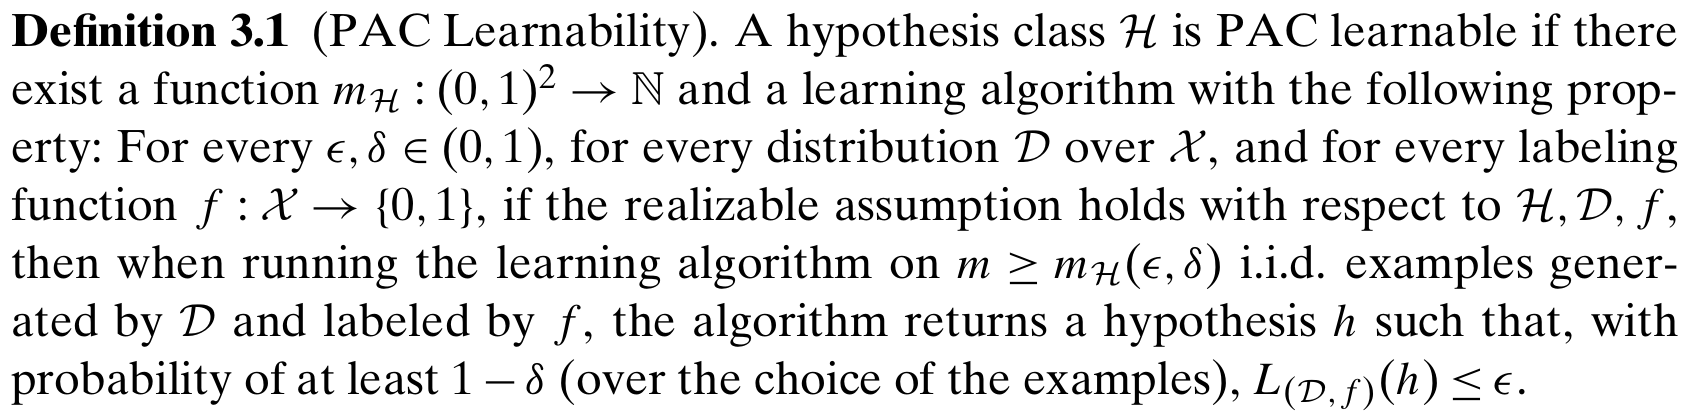
\includegraphics[width=1\linewidth]{pic/p1.png}
    \end{figure}
    A hypothesis class 
    $\mathcal{H}$ is \emph{PAC learnable} if: \\
    $\exists m_{\mathcal{H}}(\delta, \epsilon)\rightarrow \mathbb{N}$ satisfies:\\
    $\forall \epsilon,\delta\in(0,1), \{S:|S|\ge m_{\mathcal{H}}(\epsilon, \delta), S\thicksim \mathcal{D}^m\}$,\\
    $\mathbb{P}\{\exists h_S = A(S) \in \mathcal{H}, L_{(\mathcal{D}, f)}(h_S)\le \epsilon\}\ge 1 - \delta$ 
\end{frame}

\begin{frame}{Chapter2 $\sim$ Chapter3}
    \begin{figure}[h]
        \centering
        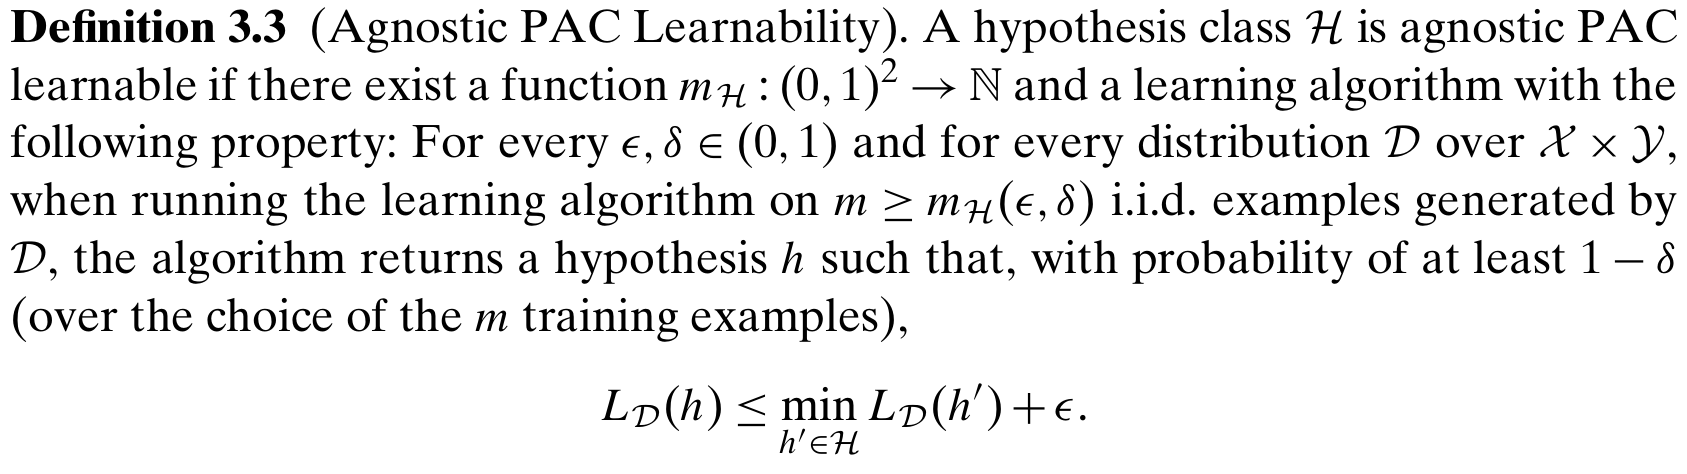
\includegraphics[width=1\linewidth]{pic/p2.png}
    \end{figure}
    A hypothesis class $\mathcal{H}​$ is \emph{agnostic PAC learnable} if:\\
    $\exists m_{\mathcal{H}}(\delta, \epsilon)\rightarrow \mathbb{N}$ satisfies:
    $\forall \epsilon,\delta\in(0,1), \{S:|S|\ge m_{\mathcal{H}}(\epsilon, \delta), S\thicksim \mathcal{D}^m\}​$\\
    $\mathbb{P}\{\exists h_S = A(S) \in \mathcal{H}, L_{\mathcal{D}}(h_S)\le\underset{h'\in\mathcal{H}}{\min}{L_\mathcal{D}(h')}+\epsilon\}\ge 1-\delta​$
\end{frame}

\begin{frame}{Chapter4 $\sim$ Chapter5}
    \begin{figure}[h]
        \centering
        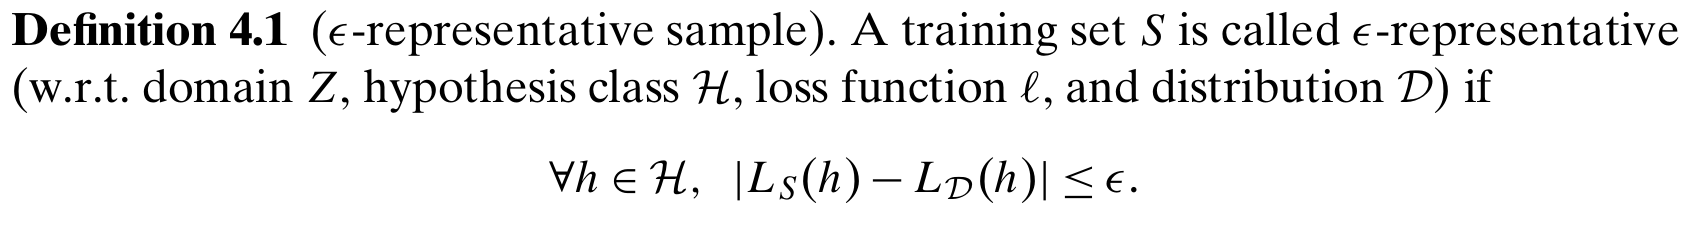
\includegraphics[width=1\linewidth]{pic/p3.png}
    \end{figure}
    \begin{figure}[h]
        \centering
        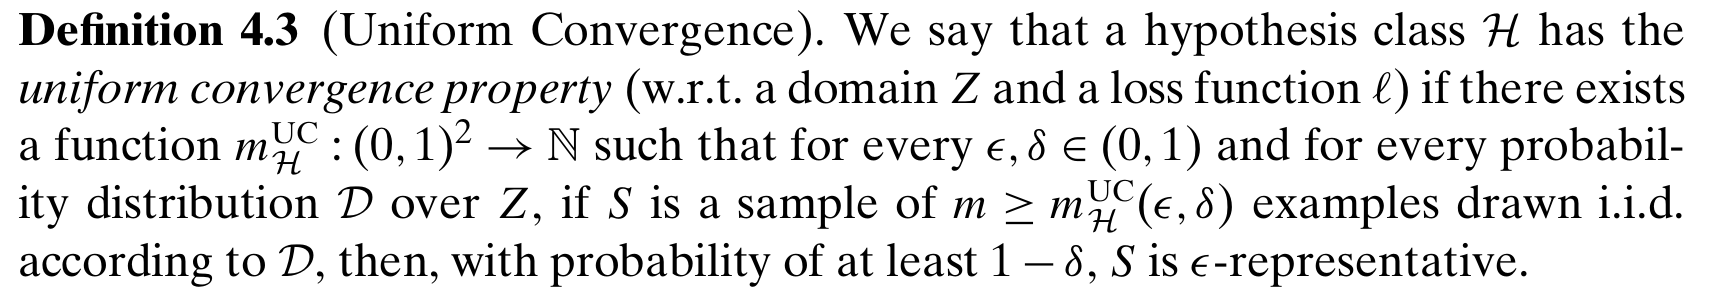
\includegraphics[width=1\linewidth]{pic/p4.png}
    \end{figure}
    A hypothesis class $\mathcal{H}​$ is \emph{Uniform Convergence} if:\\
    $\exists m^{UC}_{\mathcal{H}}(\delta, \epsilon)\rightarrow \mathbb{N}$ satisfies:
    $\forall \epsilon,\delta\in(0,1), \{S:|S|\ge m^{UC}_{\mathcal{H}}(\epsilon, \delta), S\thicksim \mathcal{D}^m\}​$\\
    $\mathbb{P}\{ \forall h \in \mathcal{H}, 
        |L_{S}(h) - L_{\mathcal{D}} (h)| \le \epsilon\}\ge 1-\delta​$
\end{frame}

\begin{frame}{Chapter6}
    \begin{figure}[h]
        \centering
        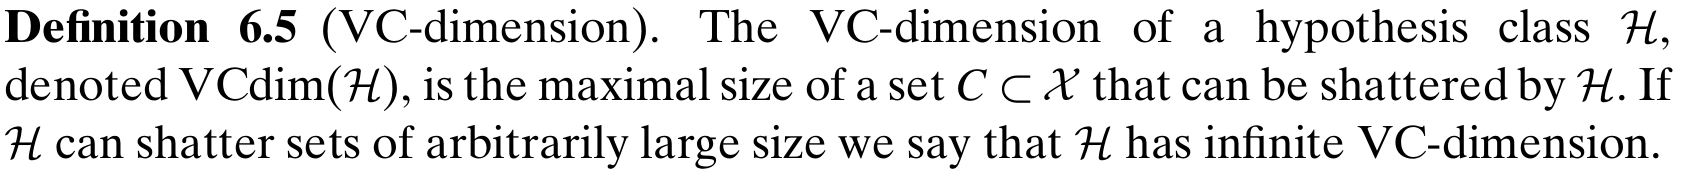
\includegraphics[width=1\linewidth]{pic/p5.png}
    \end{figure}
    \begin{figure}[h]
        \centering
        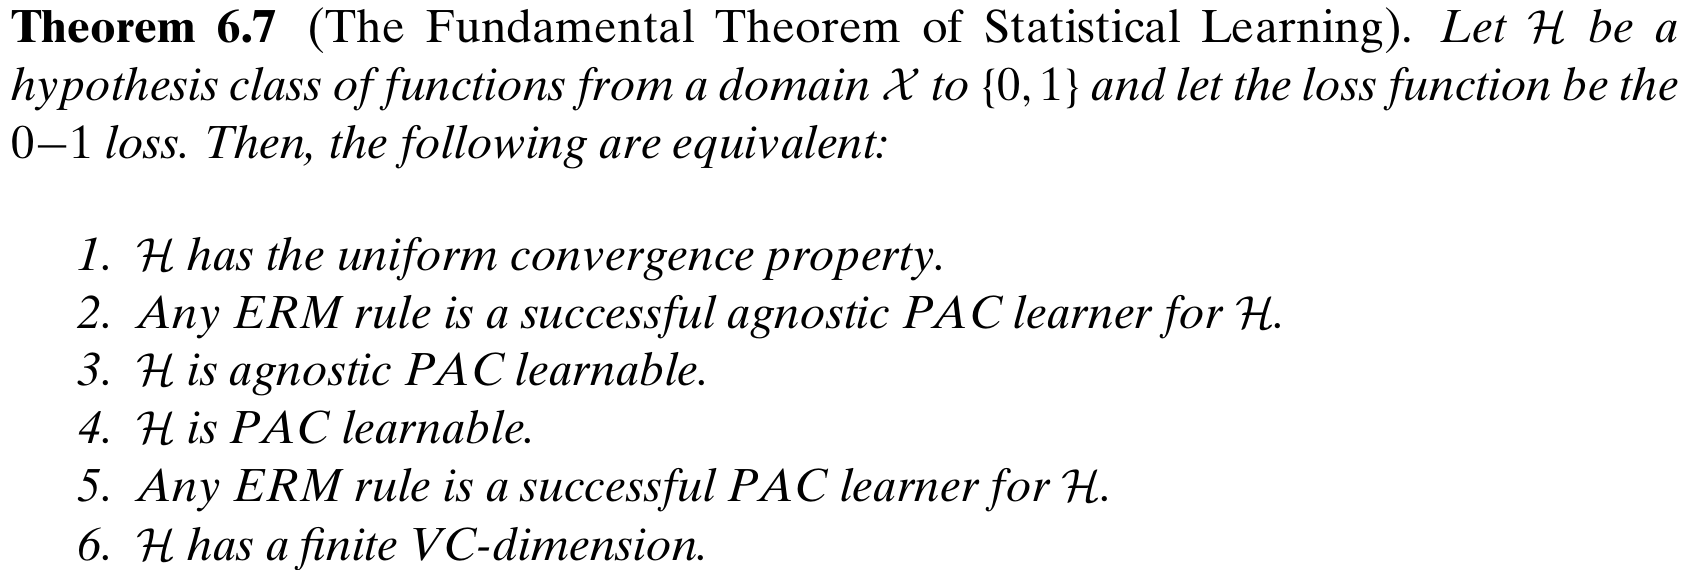
\includegraphics[width=1\linewidth]{pic/p6.png}
    \end{figure}
\end{frame}

\end{document}
